\section{Motivation}
\label{chipper:sec:motiv}

\begin{figure}[t]
	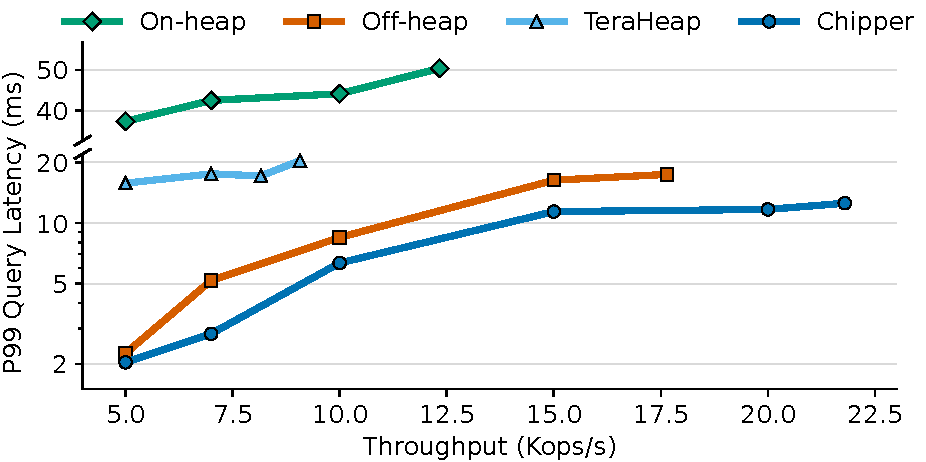
\includegraphics[width=0.5\linewidth]{chipper/figures/motiv/hbase_lat_xput_workloadc.pdf}
	\caption{P99 query latency versus achieved throughput for HBase with YCSB workload~C under the same DRAM budget.}
	\label{chipper:fig:motiv}
\end{figure}

We motivate the need for a storage-backed heap in low-pause garbage collectors using result caches of latency-sensitive applications.
We show that existing approaches either limit cache size or introduce S/D overheads that increase application tail latency.
We use HBase with YCSB~\cite{cooper:ycsb} workload~C, a read-only workload that stresses the block cache of HBase.
We show P99 query latency (Figure~\ref{chipper:fig:motiv}) of \chipperName{} against three baselines under the same DRAM budget: a DRAM-constrained on-heap cache, a storage-backed off-heap cache, and TeraHeap.
We describe the experimental baselines and methodology in \S\ref{chipper:sec:methodology}.

\paragraph{\textbf{On-heap caching is limited by DRAM.}}
The DRAM-constrained on-heap baseline sizes the block cache at 40\% of the heap, the HBase default.
As a result, the cache holds only the data that fits within the DRAM budget, and its hit rate remains at 60\% throughout the run.
Requests that miss in the cache read the corresponding blocks from storage, which dominates tail latency: P99 latency is \SI{37.8}{ms} at \SI{5}{Kops/s} and \SI{43.9}{ms} at \SI{10}{Kops/s}.
The on-heap baseline saturates at \SI{12.3}{Kops/s}, where P99 latency reaches \SI{50.4}{ms}.

\paragraph{\textbf{Off-heap caching incurs S/D cost.}}
The storage-backed off-heap baseline extends the cache beyond DRAM and can accommodate large caches.
Compared with the DRAM-constrained on-heap baseline, it reduces P99 latency by $5.2$--$16.7\times$ across load levels and sustains $1.4\times$ more throughput, reaching \SI{17.6}{Kops/s} instead of \SI{12.3}{Kops/s}.
However, HBase stores cached data blocks in serialized form, requiring deserialization and a copy into the heap on every cache hit.
S/D account for up to 30\% of the request path.
As load increases, the S/D overhead becomes more pronounced: P99 latency rises from \SI{2.3}{ms} at \SI{5}{Kops/s} to \SI{17.4}{ms} at saturation.
Moreover, the off-heap cache requires significant application modifications and extensions; applications without such support cannot extend their caches beyond DRAM without significant development.

\paragraph{\textbf{Existing storage-backed heaps have long GC pauses.}}
TeraHeap extends the managed heap to storage, avoiding both cache misses of on-heap and the S/D cost of off-heap caching.
However, TeraHeap builds on Parallel Scavenge (PS)~\cite{jones:gc_handbook}, a throughput-oriented garbage collector.
Its STW GCs limit application throughput.
The on-heap and off-heap baselines sustain $1.4\times$ and $1.9\times$ more throughput than TeraHeap, respectively.
Compared to the DRAM-constrained on-heap baseline, TeraHeap eliminates cache misses and improves P99 latency by $2.4\times$.
However, compared to the storage-backed off-heap baseline, TeraHeap has $2.4$--$7\times$ higher P99 latency due to its long GC pauses.
TeraHeap has a median GC pause of \SI{824}{ms} and a P99 GC pause of \SI{1.6}{s}, making GC the dominant source of application tail latency.

\paragraph{\textbf{Storage-backed heaps can preserve short GC pauses.}}
Each of the three baselines addresses one part of the problem but introduces another: the on-heap cache is limited by DRAM and incurs cache misses, the off-heap cache incurs S/D cost on every hit, and TeraHeap suffers from long GC pauses.
\chipperName{} is a storage-backed heap managed by a low-pause collector that addresses all three: the cache extends beyond DRAM, cache hits avoid S/D cost, and GC work remains bounded with short GC pauses.
\chipperName{} achieves up to $7\times$ lower tail latency and $1.7\times$ higher throughput than DRAM-constrained on-heap caching, transparently to the application.
